\chapter{Grundlagen}

Zunächst stellen wir die verwendete Terminologie und relevante Konzepte bzw. Phänomene dar.

\section{Kompression} \label{comp}

\subsection{Verlustfreie Kompression}
Der Prozess der Kompression überführt eine Repräsentation einer finiten Datenmenge in eine möglichst kompaktere Form. Eine verlustfreie Kompression ist gegeben, falls die Abbildung
zwischen der ursprünglichen und komprimierten Repräsentation bijektiv ist. Die Korrektheit einer verlustfreien Kompression kann daher durch die Angabe einer Dekompressionsfunktion 
nachgewiesen werden. Ist diese Vorraussetzung nicht gegeben, so handelt es sich um eine verlustbehaftete Kompression, da eine Rekonstruktion der ursprünglichen Datenmenge nicht 
garantiert werden kann.

\subsection{Eingabe}
Unsere Eingabe sei durch eine $n$-elementige Zeichenfolge $S=e_1...e_n$ über dem numerischen Alphabet $\Sigma$ mit $e_i\in \Sigma$ $\forall i=1,...,n$ gegeben. Für jede
beliebige Zeichenfolge $S$ wird mit $|S|$ dessen Länge $n$ bezeichnet. Der Ausdruck $S[i..j]\in \Sigma^{j-i+1}$ mit $1\leq i\leq j\leq n$ beschreibt die Teilfolge $e_i...e_j$ ,
wobei im Falle, dass $i=j$ ist, das einzelne Zeichen $e_i$ referenziert wird. Alternativ kann ein einzelnes Zeichen $e_i$ auch durch $S[i]$ referenziert werden. Eine Teilfolge 
der Form $S[1..k]$ mit $k\leq n$ wird als Präfix von $S$ bezeichnet.

\subsection{Faktorisierung}
Ein charakteristisches Merkmal für die Klasse von Lempel-Ziv-Kompressionsverfahren ist die Repräsentation der Ausgabe in Form einer Faktorisierung. Für eine Eingabe $S=e_1...e_n$ 
wird eine Faktorisierung $F=f_1...f_z$ mit $z\leq n$ derart erzeugt, dass die Faktoren $S$ in eine equivalente Folge von nichtleeren Teilfolgen zerlegen. Hier ist jeder Faktor
$f_i$ mit $1\leq i\leq z$ als Präfix von $S[|f_1...f_i-1|+1..n]$ definiert, der bereits in $S[1..|f_1...f_i|]$ vorkommt oder als einzelnes Zeichen ohne vorheriges Vorkommen. Die im 
Folgenden betrachteten Algorithmen können speziell der Klasse der LZ77-Kompressionsverfahren zugeordnet werden, dessen Faktoren im Schema des Lempel-Ziv-Storer-Szymanski repräsentiert
werden sollen. Zur Darstellung von Referenzen wird das Tupel $(len, pos)$ verwendet, wobei $pos$ die Position des vorherigen Vorkommens und $len>0$ die Länge des Faktors beschreibt. 
Einzelne Zeichen können wiederum durch das Tupel $(0, e)$ mit $e\in \Sigma$ dargestellt werden.

\subsection{Dekompression}
Die Dekompression beschreibt den Umkehrprozess der Kompression und erlaubt im Falle eine verlustfreien Kompression die Rekonstruktion der ursprünglichen Datenfolge. Im Falle von 
Verfahren der LZ77-Familie, kann die Dekompression durch die folgende Abbildung definiert werden, 
\begin{equation}
    DECOMP_{LZ77}: F(1..z) \rightarrow S(1..n).
\end{equation}

\begin{algorithm}
\centering
\caption{DECOMP$_{LZ77}$} \label{alg:decomp}
\algorithmicrequire $F=f_1...f_z$
\algorithmicensure $S=e_1...e_n$
\begin{algorithmic}
    \STATE $S \gets \emptyset$
    \FOR{$i=1$ to $z$}
        \STATE [len, ref] $\gets f_i$
        \IF{len = 0} 
            \STATE $S \gets S + ref$
        \ELSE
            \FOR{$j=0$ to $len-1$}
                \STATE $S \gets S + S[ref + j]$
            \ENDFOR
        \ENDIF
    \ENDFOR
    \RETURN $S$
\end{algorithmic}
\end{algorithm}

Der dargestellte Algorithmus \ref{alg:decomp} beschreibt eine mögliche Implementierung der Dekompression für eine Faktorisierung $F=f_1...f_z$ zu der Eingabe $S=e_1...e_n$.
Der beschriebene Algorithmus iteriert durch alle Faktoren und fügt die referenzierten Zeichen einzeln in die Ausgabe $S$ ein. Damit kann die Laufzeit des Algorithmus auf $O(n)$
geschätzt werden.

\subsection{Verlustbehaftete Kompression}
Im Rahmen dieser Arbeit werden einen Approximationsalgorithmus betrachten, der aufgrund der verwendeten String-Matching-Technik eine fehlerhafte Faktorisierung mit einer 
beschränkten Wahrscheinlichkeit erzeugen kann. Die Korrektheit der Dekompression kann intern und extern durch explizite Vergleiche der Zeichenfolgen erkannt werden. Da der
Kompressionsprozess in diesem Fall mit anderen Parametern wiederholt werden kann, können wir einen verlustfreien Las-Vegas-Algorithmus konstruieren.

\begin{figure}
    \centering
    \caption{Las-Vegas-Algorithmus}
    \label{fig:lasvegas}
    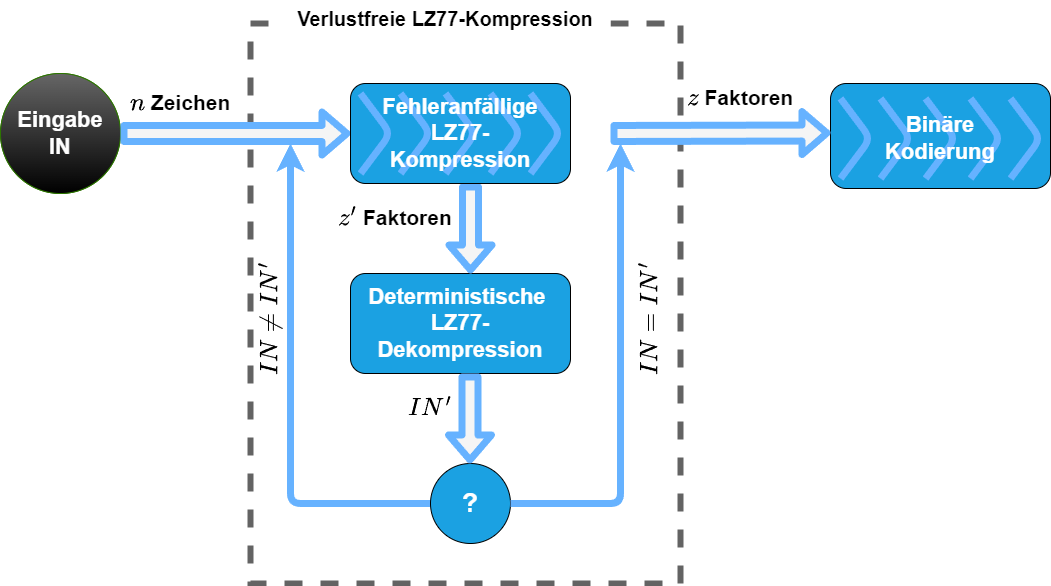
\includegraphics[scale=0.25]{bilder/lasvegas_algorithm.png}
\end{figure}

In Abbildung \ref{fig:lasvegas} wird die beschriebene Schleife illustriert. Der Algorithmus wird solange wiederholt, bis eine korrekte Faktorisierung erzeugt wurde. Dass die
Anzahl der Wiederholungen beschränkt ist, werden wir in der Analyse des Approximationsalgorithmus und der praktischen Evaluation zeigen.

\subsection{Binäre (De-)Kodierung}
Die Abbildung $Bin_{IO}: \Sigma^* \rightarrow N$ gibt die Anzahl der Bits für die Kodierung einer beliebigen Zeichenfolge an. Im Rahmen dieser Arbeit gehen wir davon aus, dass die 
Eingabe $S$ in binärer Form vorliegt und auf dem Alphabet $\Sigma=\{1,...,255\}$ erzeugt wurde. Jedes Zeichen wird durch 8 Bits, oder 1 Byte, dargestellt und erlaubt einen 
Offline-Zugriff. Die gesamte binäre Eingabegröße sei damit gegeben durch 

\begin{equation}
    N_{Bin} = \sum_{i=1}^{|S|} Bin_{IO}(S[i]) = 8*|S|.
\end{equation}
Die eingelesene Eingabefolge wird durch den Kompressionsalgorithmus in die Faktorfolge $S=f_1...f_z$ überführt. Jeder Faktor $f_i$, der Form $(len, pos)$ oder $(0, e)$, werde 
durch $Bin_{IO}(f_i)$ Bits kodiert. Die binäre Ausgabegröße ergibt sich aus dem Ausdruck
\begin{equation}
    Z_{Bin} = \sum_{i=1}^{z} Bin_{IO}(f_i).
\end{equation}
, wobei die Anzahl der Bits für die Kodierung der Faktoren $f_i$ durch den Kompressionsalgorithmus und der Kodierungsstrategie bestimmt wird. 

\subsection{Metriken}
Die Qualität einer Kompression kann durch verschiedene Metriken quantifiziert werden. Zum Einen beschreibt die Kompressionsrate $CR$ den Grad der Kompression und ist durch den
Ausdruck, 
\begin{equation}
    CR = \frac{Z_{Bin}}{N_{Bin}}
\end{equation}
, definiert.
Da die Kodierung der Faktoren nicht eindeutig aus der Wahl des Kompressionsalgorithmus eingegrenzt wird, ist stattdessen die Anzahl der erzeugten Faktoren ein
weiteres geeignetes Gütemaß. Für die Eingabe $S$ der Länge n und der Ausgabe $f_1...f_z$ sei die Faktorrate durch
\begin{equation}
    FR = \frac{z}{n}
\end{equation}
gegeben. In beiden Fällen wird ein niedriger Wert bevorzugt, da dieser auf eine bessere Extraktion von Redundanzen hinweist.

\section{Parallelität}
Das Ziel dieser Arbeit ist die Entwicklung und Evaluation eines parallel Kompressionsalgorithmus. Im Folgenden definieren wir die Rahmenbedingungen und Konzepte der Parallelität.

\subsection{Shared-Memory-Modell}
Unser Algorithmus agiere auf einem Shared-Memory-Modell mit $P$ Ausführungseinheiten, welches im Gegensatz zum Distributed-Memory-Modell allen beteiligten Ausführungseinheiten bzw. 
Prozessoren einen gemeinsamen Zugriff auf den Speicher ermöglicht. Im Rahmen der Arbeit und Kommunikation unter den Prozessoren wird man jedoch auf Konflikte bei gleichzeitigen 
Speicherzugriffen zustoßen. Ein parallel modellierter Algorithmus muss explizit hinsichtlich der Korrektheit und Effizienz Mechanismen zur Synchronisation implementieren.

\subsection{Metriken}
Das Ziel der Parallelisierung eines Algorithmus liegt hauptsächlich in einer Verbesserung der Laufzeit, insbesondere unter Berücksichtigung von Ressourcenkonflikten. Die zeitliche
Beschleunigung der Laufzeit kann durch den Speedup $SP$ bemessen werden. Für eine Eingabe $S$ der Länge n brauche ein sequenzieller Durchlauf $T(n, p=1)$ Zeit, während ein paralleler
Algorithmus mit $P$ Prozessoren $T(n,p=P)$ an Zeit benötigt. Der Speedup ist dabei definiert durch
\begin{equation}
    SP(n,P) = \frac{T(n,1)}{T(n,P)}.
\end{equation}

